\documentclass[11pt]{article}
\usepackage{graphicx,tabularx}
\usepackage{amssymb}
\usepackage{amsmath}
\usepackage{hyperref}
%\usepackage{draftwatermark}
\usepackage[small,scriptsize]{caption}
\usepackage{fancyhdr}
\newcommand{\Cerenkov}{\v{C}erenkov}
\newcommand{\degrees}{$^\circ$}
\newcommand{\NN}{$\mathrm{N_2}$}
\newcommand{\CF}{$\mathrm{C_4F_{10}}$}
\newcommand{\CO}{$\mathrm{CO_2}$}
\newcommand{\OO}{$\mathrm{O_2}$}
\newcommand{\MgF}{$\mathrm{MgF_2}$}
\newcommand{\KCsSb}{$\mathrm{K_2CsSb}$}
\newcommand{\GaP}{$\mathrm{GaP(Cs)}$}
\newcommand{\dray}{$\delta\mathrm{-ray}$}
\newcommand{\tr}[1]{\mathrm{Tr}\left\{#1\right\}}
\newcommand{\Real}[1]{\mathrm{Re}\left\{#1\right\}}
\newcommand{\Imag}[1]{\mathrm{Im}\left\{#1\right\}}
\newcommand{\be}{\begin{enumerate}}
\newcommand{\ee}{\end{enumerate}}
\newcommand{\bi}{\begin{itemize}}
\newcommand{\ei}{\end{itemize}}


\pagestyle{fancy}
\headheight 35pt


\begin{document}

%\section{}
%\subsection{}



\subsection{Super HMS Noble Gas Cerenkov Detector}
Analyzing momenta up to
11~GeV/c at scattering angles from 5.5 to 40.0  degrees, the SHMS will reach
kinematic regions in which the pion background  rate dominates the scattered electron
rate by more than 1000:1.  The  suppression of these anticipated pion backgrounds
while maintaining efficient identification of electrons  is therefore one
of the main duties of  the SHMS detector elements and the SHMS Noble Gas \Cerenkov\ Detector shoulders a large portion of this particle identification burden.
The design of the  noble gas threshold \v Cerenkov
detector is such that it will meet these twin goals of suppression and identification.
The main goal of the detector is to distinguish between electrons and pions with momenta between 6 GeV and 11 GeV/c. 

The basic equation  governing \v Cerenkov radiation emitted by a particle 
of velocity $\beta$ traveling through a medium with index of refraction
$n$ is \begin{equation}\cos \theta = \frac{1}{\beta n},\end{equation}
where $\theta$ is the angle of the \v Cerenkov light cone.
From this it is easy to see that for there to be any radiation
$$n > 1/\beta.$$
What we need is that 
\begin{equation} n < 1/\beta_{\pi,max}\label{eq:index} \end{equation}
to guarantee that the pions produce no radiation directly, and that
\begin{equation} n > 1/\beta_{e^-,min} \end{equation}
to guarantee that all the electrons produce  Cerenkov light. Since
$1/\beta_{e^-,min} < 1/\beta_{\pi,max}$, we need to use only one value of $n$
over the planned momentum range. Figure~\ref{fig:partsep}  emphasizes this point with a plot of the hadron velocity (given as $(1-\beta)$) as a function of momentum along with the lines indicating the index of refraction  of various gases at 1 atm, as $(n-1)$.  For a threshold Cerenkov counter only those particles with $(1-\beta) < (n-1)$ will produce light. For example no $\pi$'s with momenta less than 6 GeV/c will produce Cerenkov radiation in 1 ATM of Argon. If the $\pi$'s momenta exceed 6 GeV/c then it will cross the `threshold' and Cerenkov radiation will be emitted.
 \begin{figure}[!h] %  figure placement: here, top, bottom, or page
   \centering
   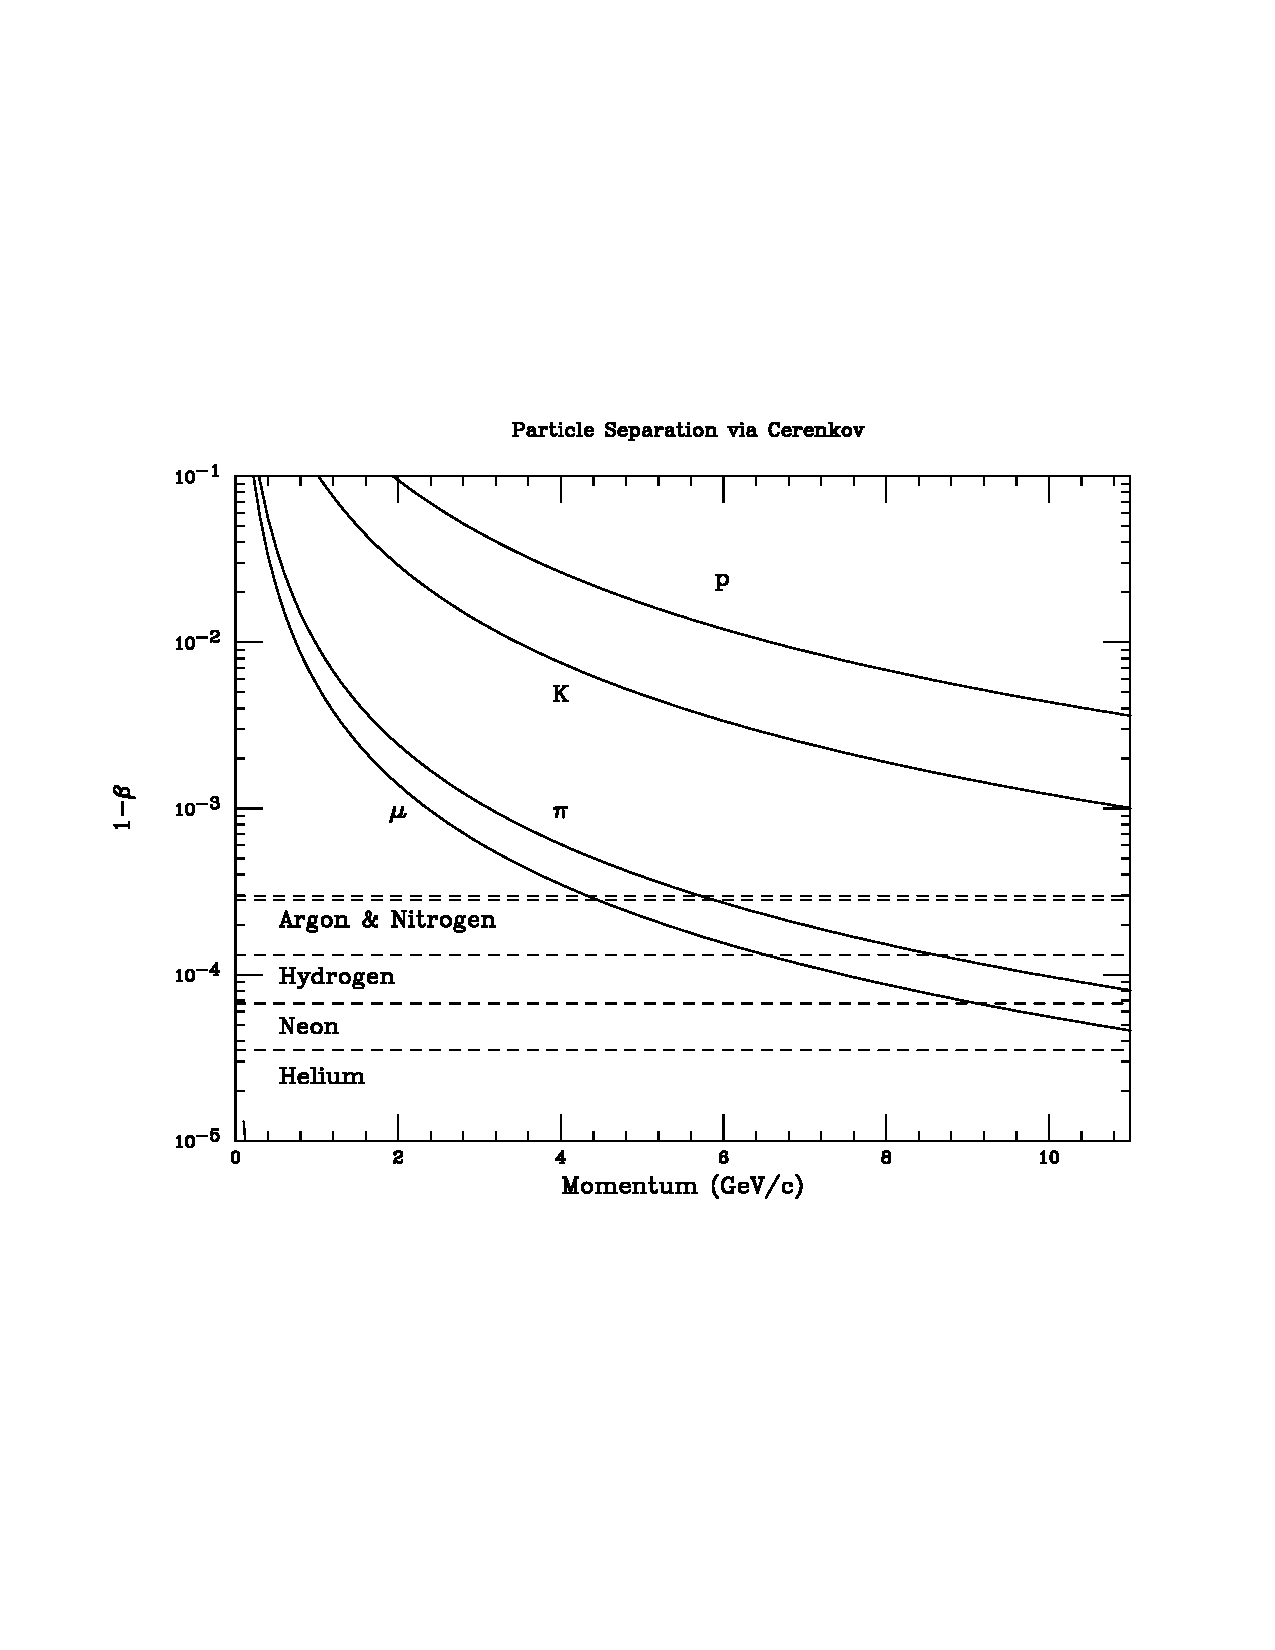
\includegraphics[width=0.8\textwidth]{./Figures/partsep} 
   \caption{Particle identification with a threshold Cerenkov detector. Plotted is the hadron velocity as $(1-\beta)$ against the hadron momenta. The horizontal lines indicate, for different gases at 1 ATM, the index of refraction as $(n-1)$. Only when $(1-\beta)$ is less than $(n-1)$ does the particle produce light.}
   \label{fig:partsep}
\end{figure}
A first glance at Fig.~\ref{fig:partsep} indicates that Neon would be a good choice for the SHMS Cerenkov detector. Operation at 1 ATM  allow the windows on the detector tank to be very thin.

It is also possible to use a mixture of gases to fine tune the index of refraction and improve the detector performance. In this case the weighting of the index of refraction of the different gases is by the number of molecules per unit volume for each gas and the index is linear in  the number per unit volume for each species. It should be possible to obtain pre-mixed gases from a vendor or mix them using techniques already in use at the laboratory. Hence the device has been designed to use Argon and Neon a the limits of 6 GeV/c and 11 GeV/c and a mixture in between.


The SHMS HGC design was restricted by the available space and the need to have good discrimination at the highest momenta.  The number of photoelectrons is maximized in this design by the use of quartz window PMTs and mirrors with excellent reflectivity well into the UV. See Fig.~\ref{fig:tubeandmirror}. It was also desired to have a minimum of  material in the path of the charged particles on order  to keep multiple scattering small and preserve  the SHMS design resolutions. The materials crossed by charged particles can be found in  Fig.~\ref{fig:materials}.

\newpage
\vspace{.25in}
\noindent {\bf Description of the Cerenkov}
\vspace{.25in}

The NGC consists of the following elements:
\be
\item 2m long tank fabricated with an internal rigid frame and thin aluminum walls welded together. See Fig.~\ref{fig:Box}.

 The tank has an active volume of 2m along the beam direction and approximately 90 cm tank perpendicular to the beam direction. The tank was designed to position the PMTs outside the active area. The main access is provided through a large 'door' and  four small panels provide modest access to the PMTS. There are large entrance and exit windows. The detector will operate at 1 ATM of either Argon or Neon or a mixture of the two. The tank has feed throughs for   gas management as well as for  HV and signal cables. A black flat paint has been applied to the interior of the tank to prevent the reflection of light from cosmic rays or hall background. 

\item Four spherical thin glass mirrors of radius 135 cm, square in shape with  edges of 43cm.

  The mirrors overlap in the center to provide full coverage of the active area and each focus the reflected Cerenkov light on a separate PMT. The mirrors are tilted by 15$^\circ$ to allow the PMTs to be outside he active area.
The mirrors are positioned in a monolithic frame that is installed as single unit. The mirrors are installed, the overlap set and rotated with the frame on a table outside the tank.  See~Fig.\ref{fig:install}.
\item Four 14~stage 5~inch quartz window PMTs manufactured by Electron Tubes Enterprises.

 The PMTs are model 9823QKB04 and  tubes with serial numbers 16747, 16777, 16787 and 16785 are installed to accept light from the mirrors in position Top Right, Top Left, Bottom Right and Bottom Left respectively while looking along  increasing $z$. The tubes are surrounded by a mu-metal shield and the HV is distributed to the stages by a positive base.
\item Thin entrance and exit window made of two layers of 2 mils of the Dupont product, Tedlar  - (CH$_2$CHCl)$_n$.
\ee
\begin{figure}[!h] %  figure placement: here, top, bottom, or page
   \centering
   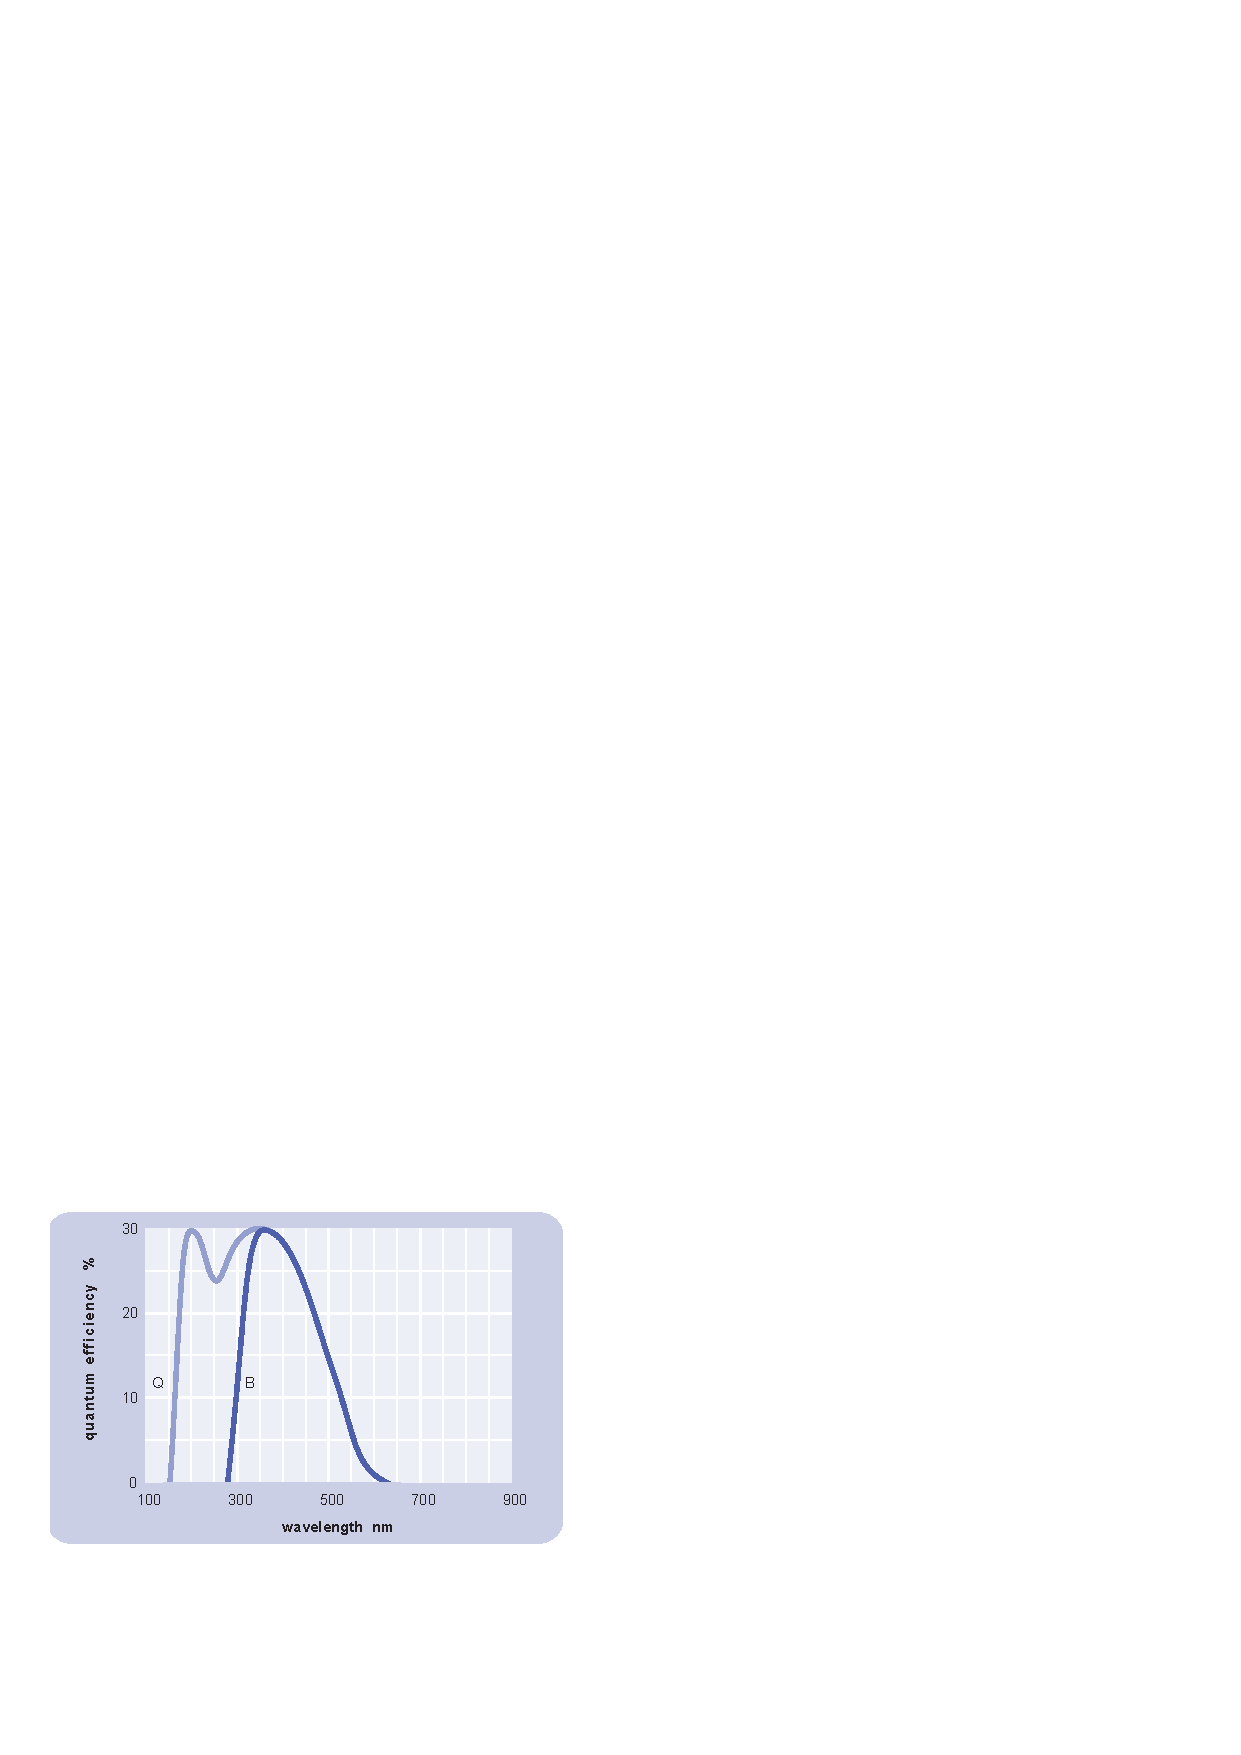
\includegraphics[width=.45\textwidth]{./Figures/9832BQ} 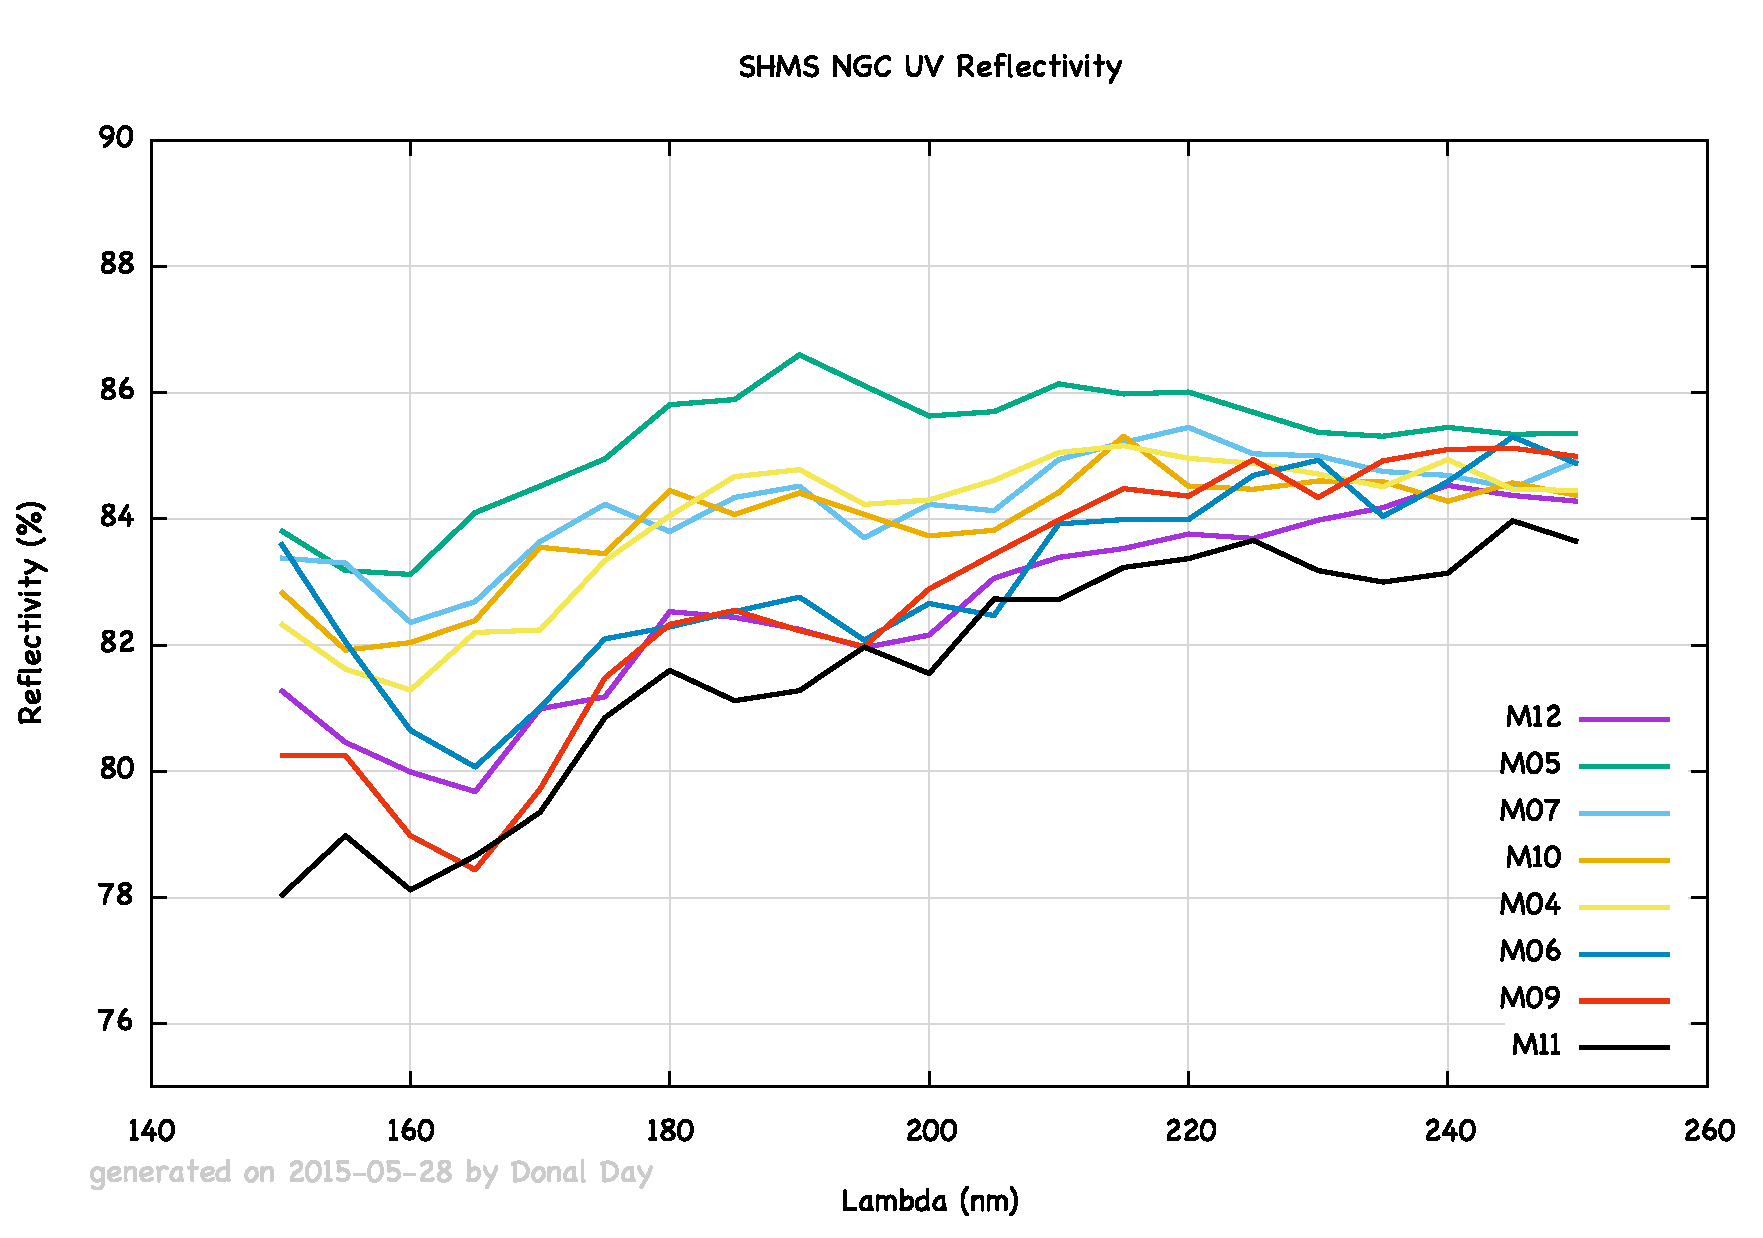
\includegraphics[width=.45\textwidth]{./Figures/UVReflcectanceCERN}    \caption{LHS: Quantum efficiency of Electron Tubes Enterprises model 9823QKB04 - light blue curve, labelled ``Q". RHS: The UV measured reflectivity of the mirrors  coated at CERN. Between 250 nm and 600 nm the reflectivity rises to almost 90\%. \label{fig:tubeandmirror}}
   
   \end{figure}
 \begin{figure}[!h] %  figure placement: here, top, bottom, or page
   \centering
   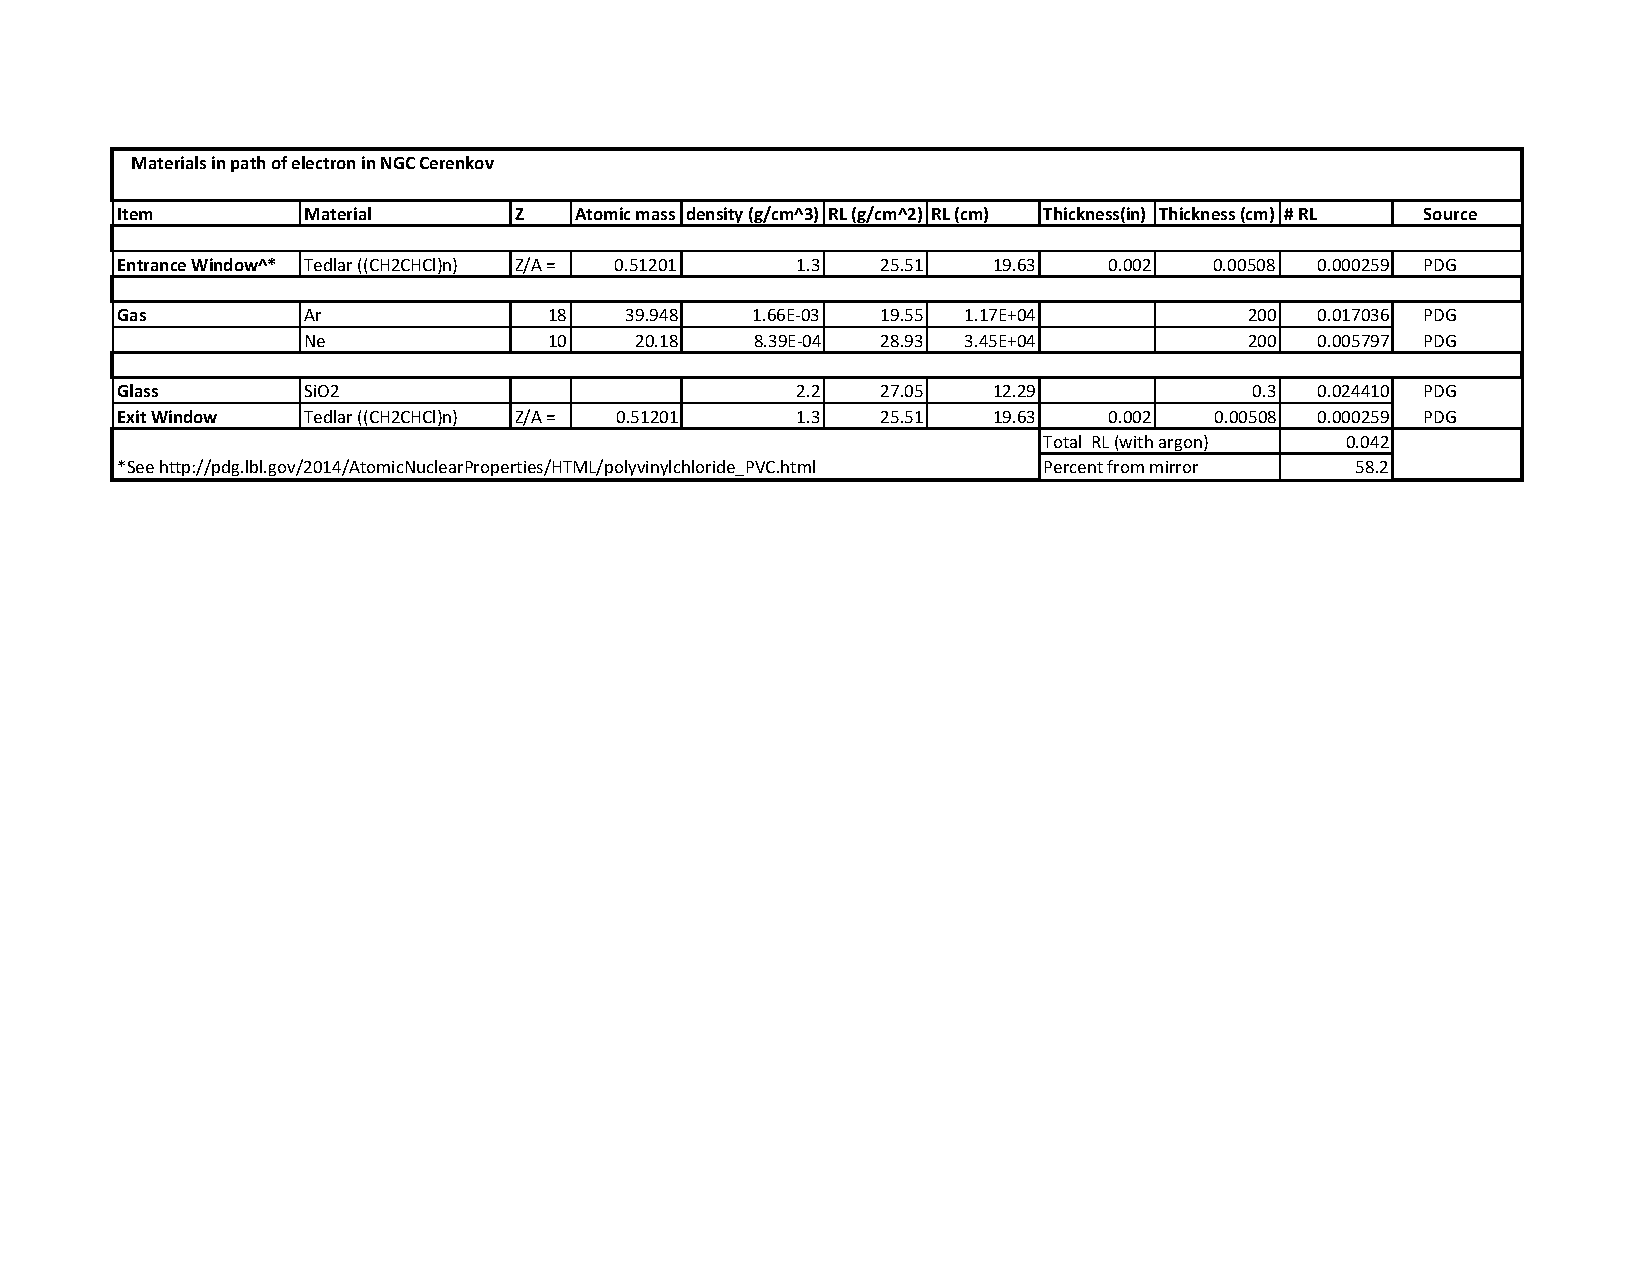
\includegraphics[width=\textwidth]{./Figures/MaterialsinCerenkovFeb2016Crop}    \caption{Materials in the path of charged particles passing through the NGC.\label{fig:materials}}
   \end{figure}



\begin{figure}[!h] %  figure placement: here, top, bottom, or page
   \centering
   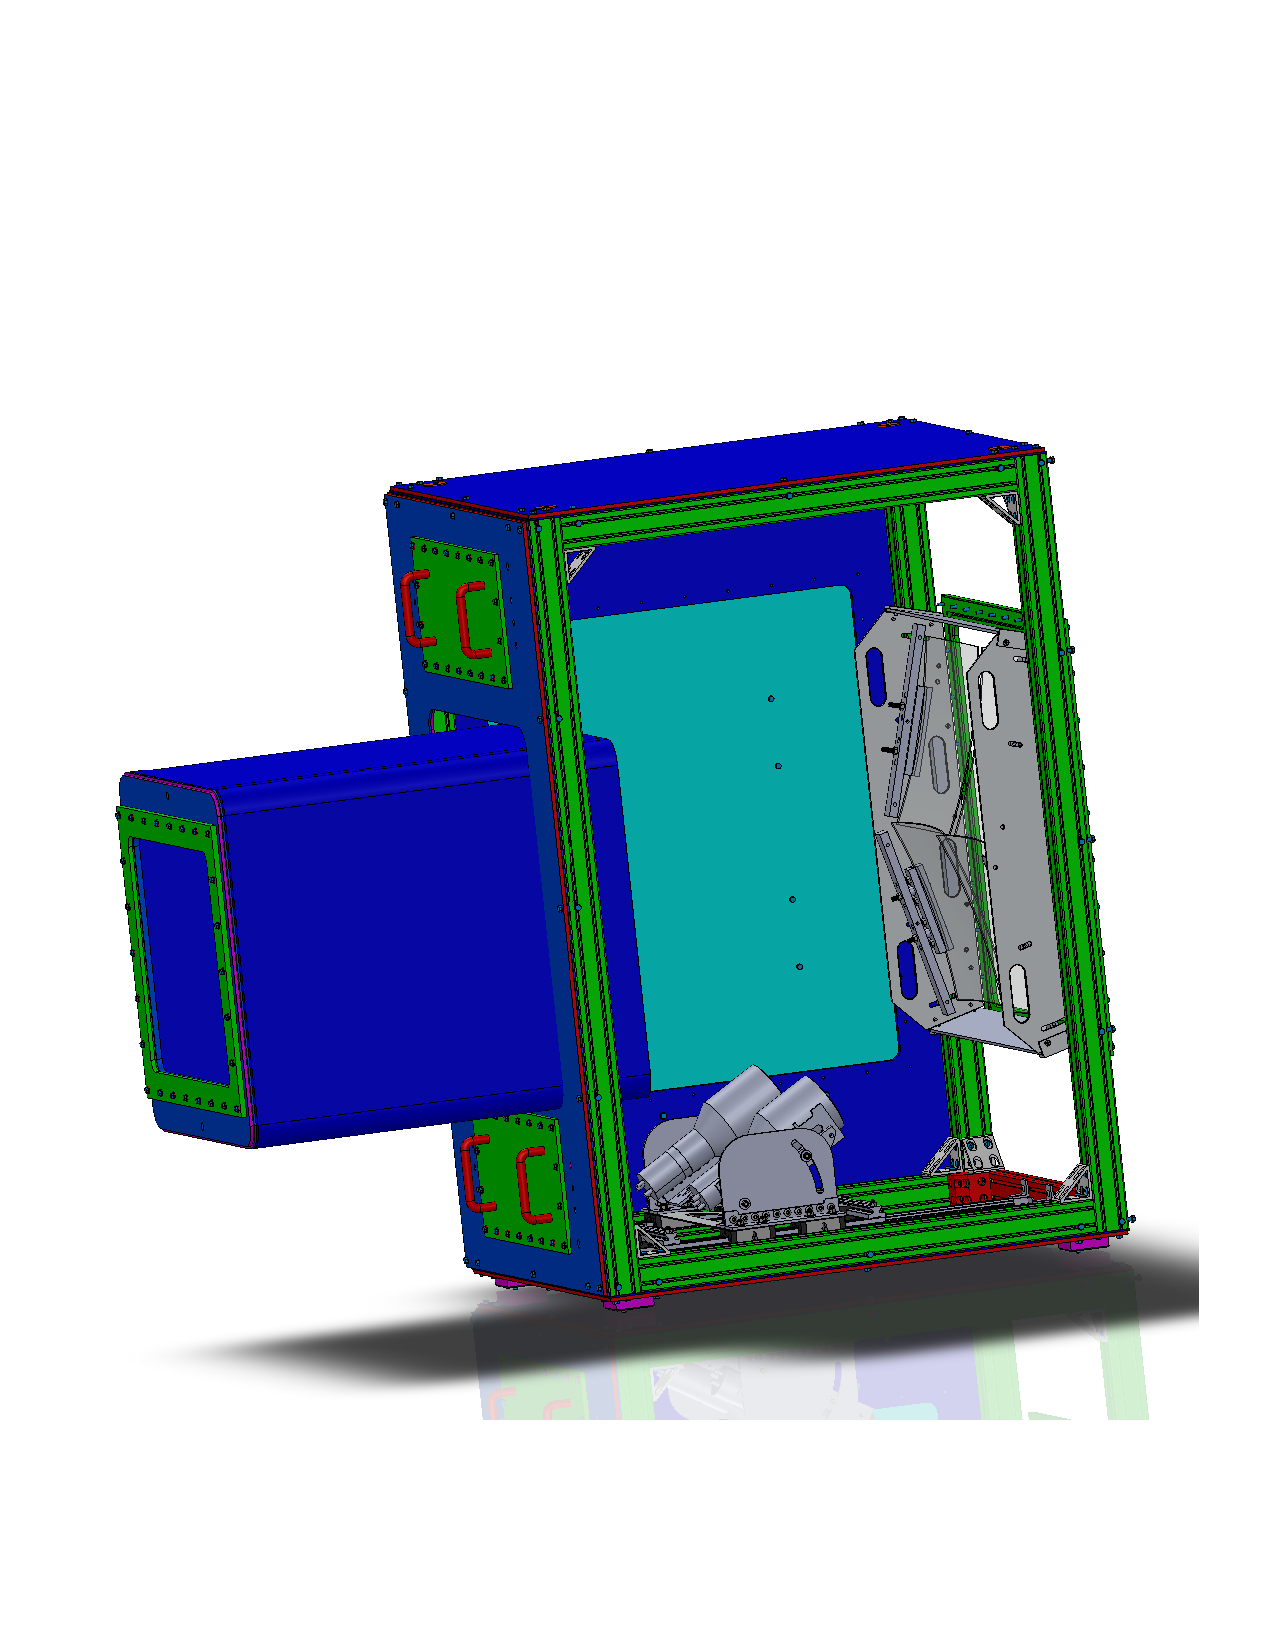
\includegraphics[width=0.45\textwidth]{./Figures/z1FullConstruction_easmCrop.pdf} 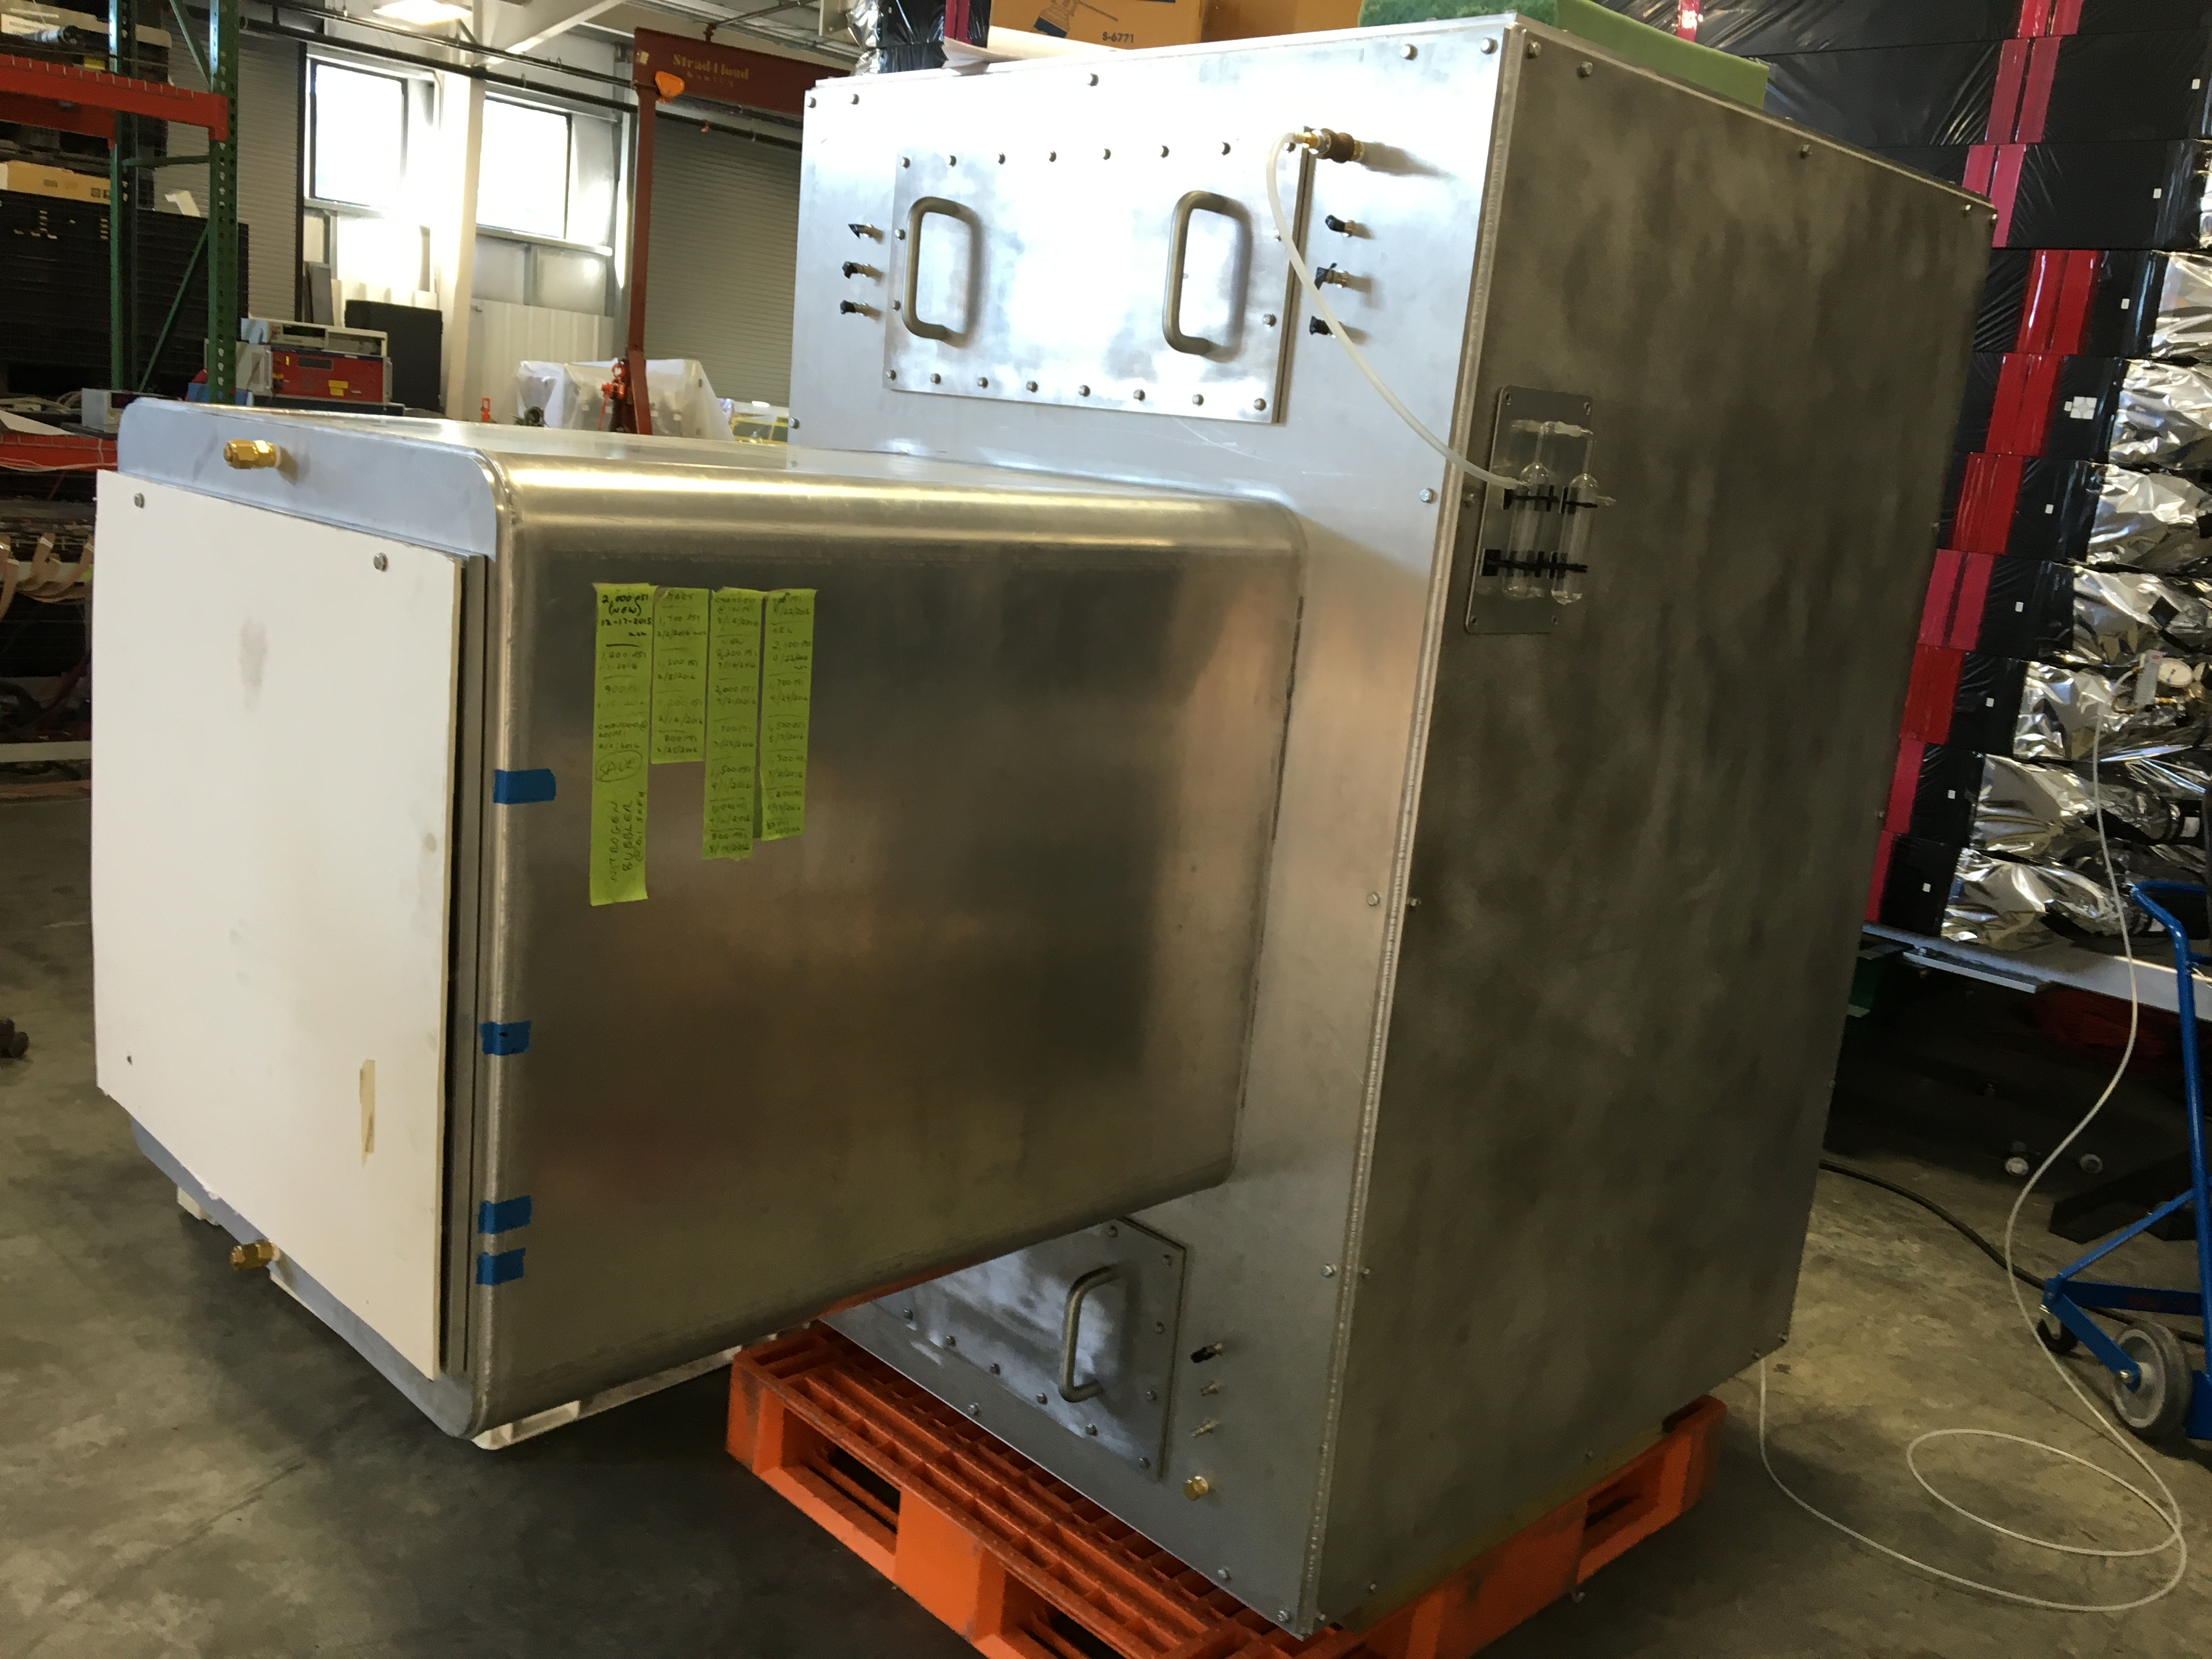
\includegraphics[width=0.45\textwidth]{./Figures/TankAsBuilt} 
   \caption{LHS: Sketch of the NGC tank. This view is possible as one panel is removed. Note the PMT mounting system is different than shown here.  RHS: Buttoned up tank waiting installation.\label{fig:Box}}
 
\end{figure}

\vspace{.25in}
\noindent {\bf{Gas Filling Procedure - to be added}}
\vspace{.25in}

The tank contains four 5 inch PMT's which use {\bf positive} HV. They operate
at between 1900 and 2400 Volts. The Anode is at HV and its signal is
viewed through a decoupling capacitor in the base. {\bf TBD: The HV is supplied
by one pod of the same {\em CAEN} power supply used for the drift chambers.}

The mirrors in the tank may require adjustment for optimal focusing
on the PMT faces. This is only possible when the tank is out of the SHMS and on a horizontal surface (the hall floor)  and the access door removed  allowing entry into the tank. The tank is a confined
space and hence this activity represents an ODH hazard. Stickers indicating
this have been placed on the PMT ports and on the door. Before an entry into the tank the
atmosphere in the interior must be surveyed by a member of the physics
division EH$\&$S staff.
This adjustment should only be done by personnel with experience. A document, ``NGC Mirror Installation and Tuning'',  has been written describing the optical tuning and it can be found at \url{https://hallcweb.jlab.org/doc-private/ShowDocument?docid=794}

\begin{figure}[!h] %  figure placement: here, top, bottom, or page
   \centering
   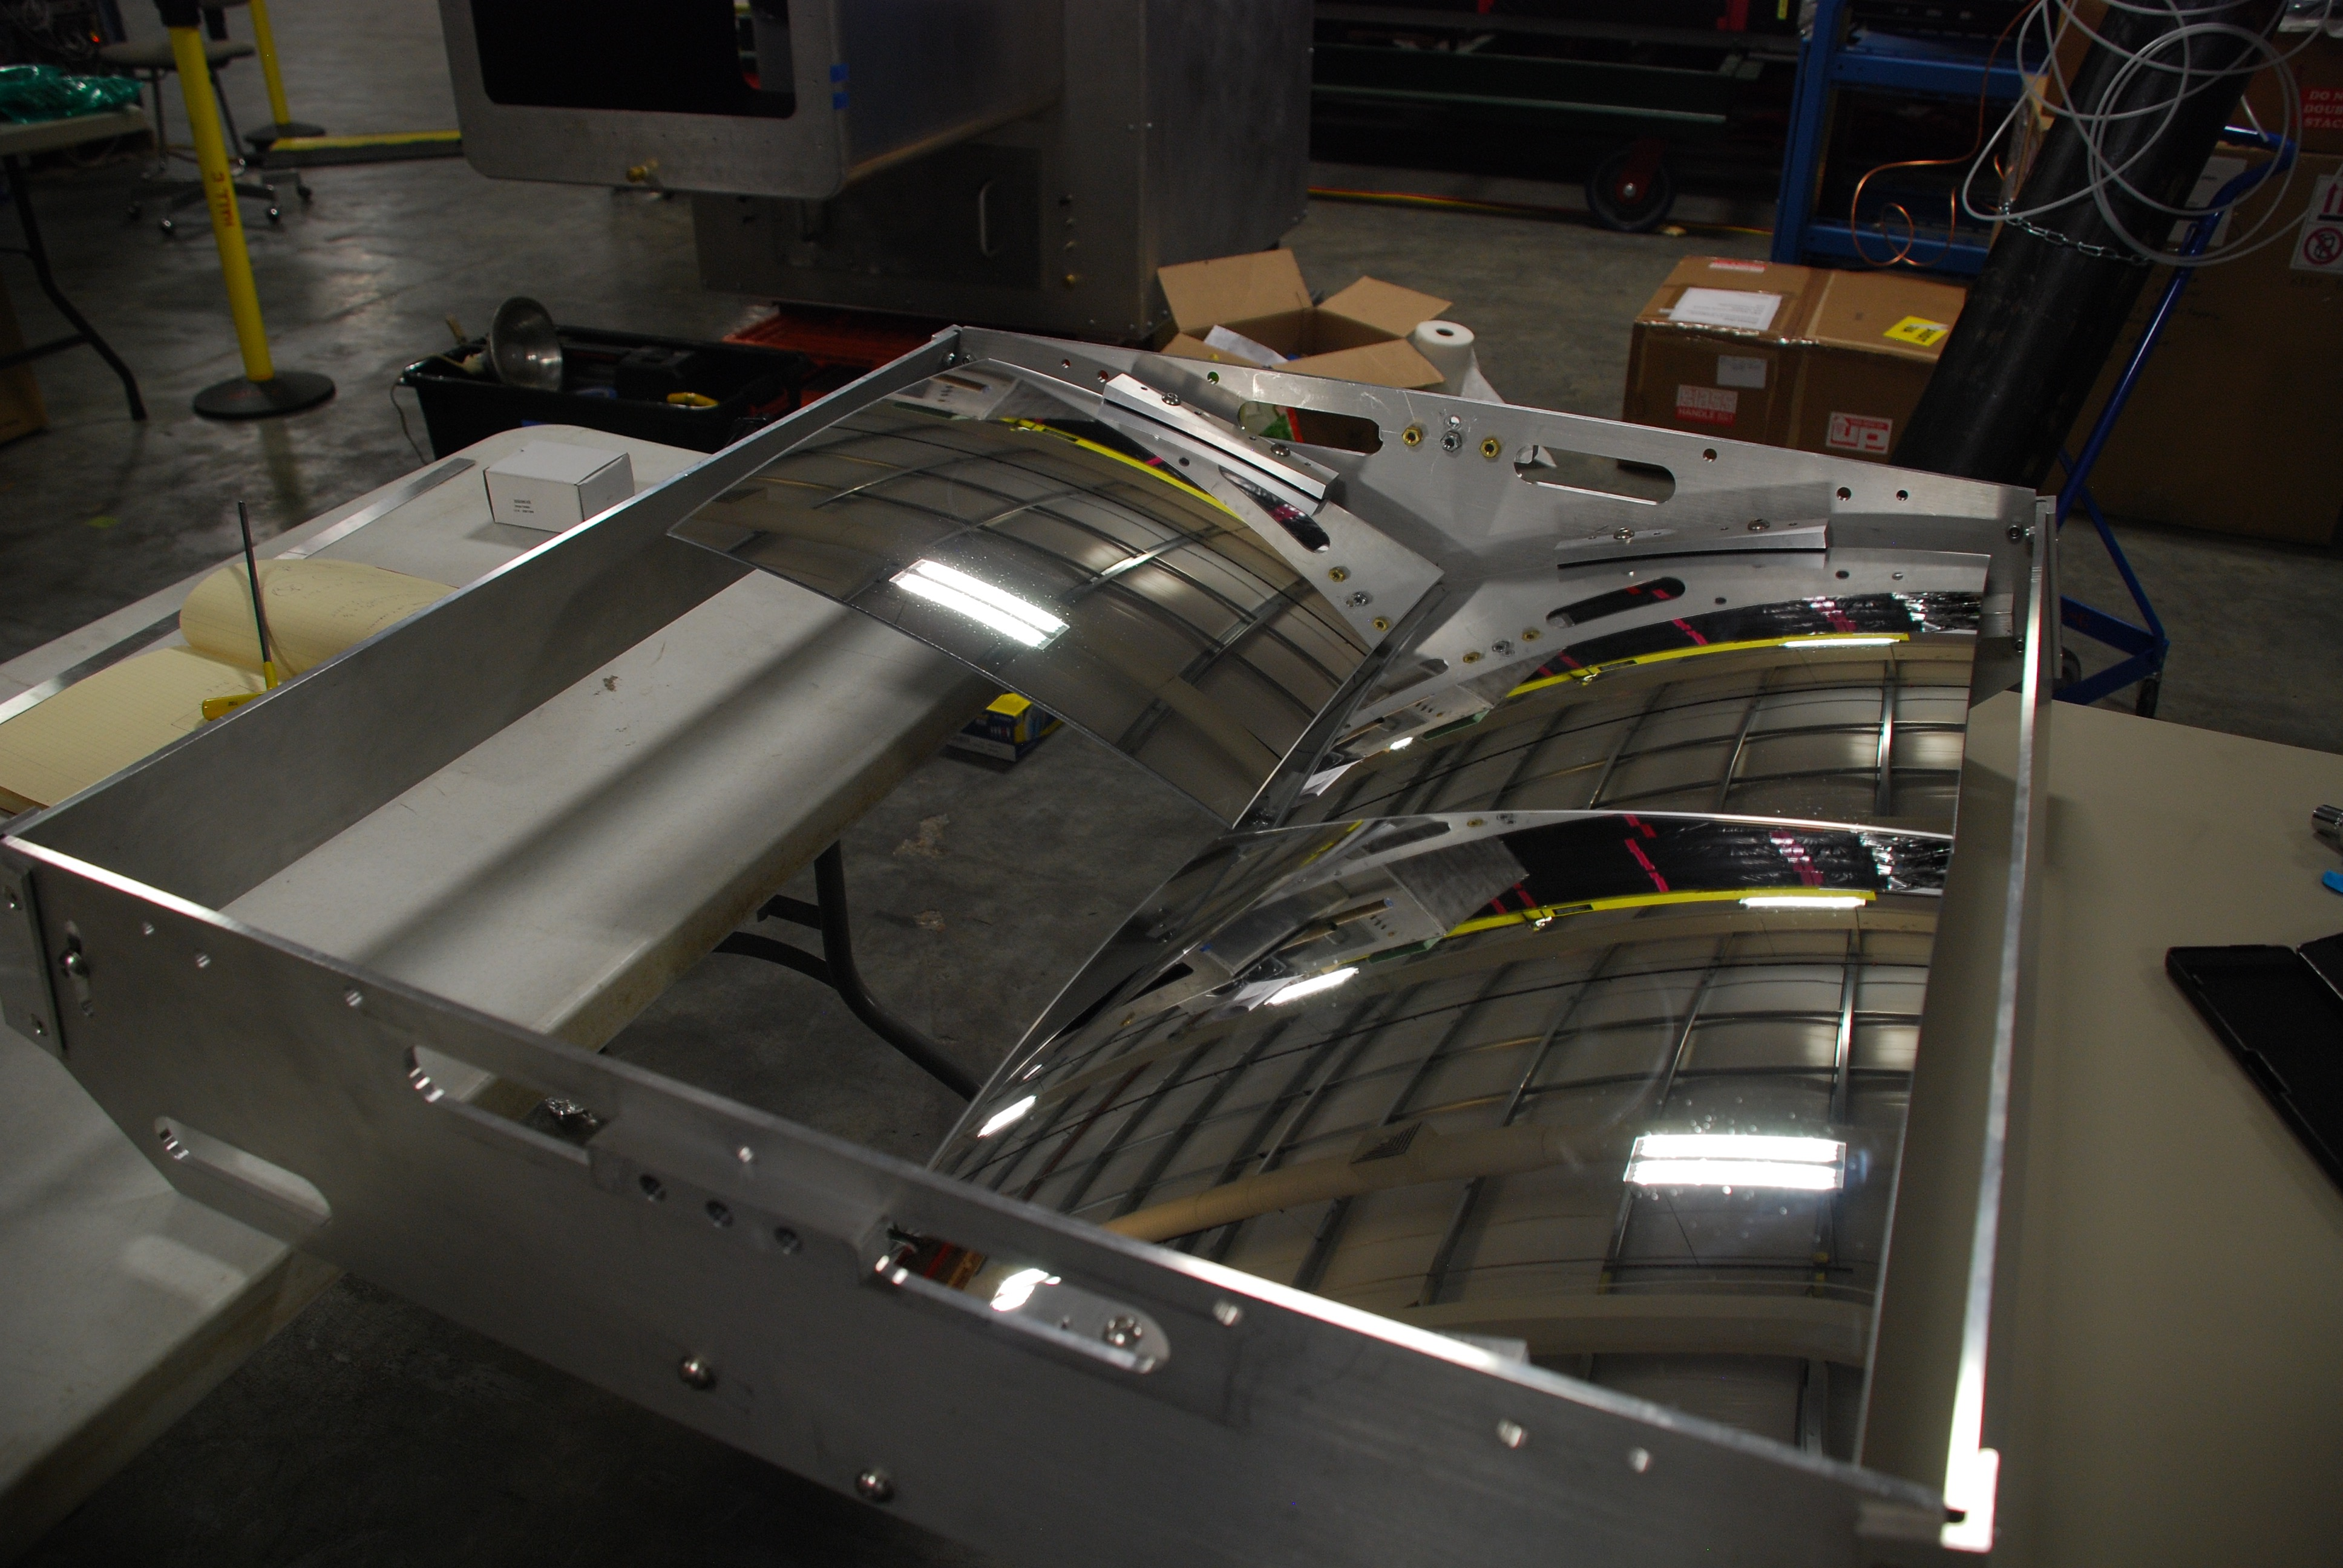
\includegraphics[width=0.45\textwidth]{./Figures/TwoMirrorsinFrame} 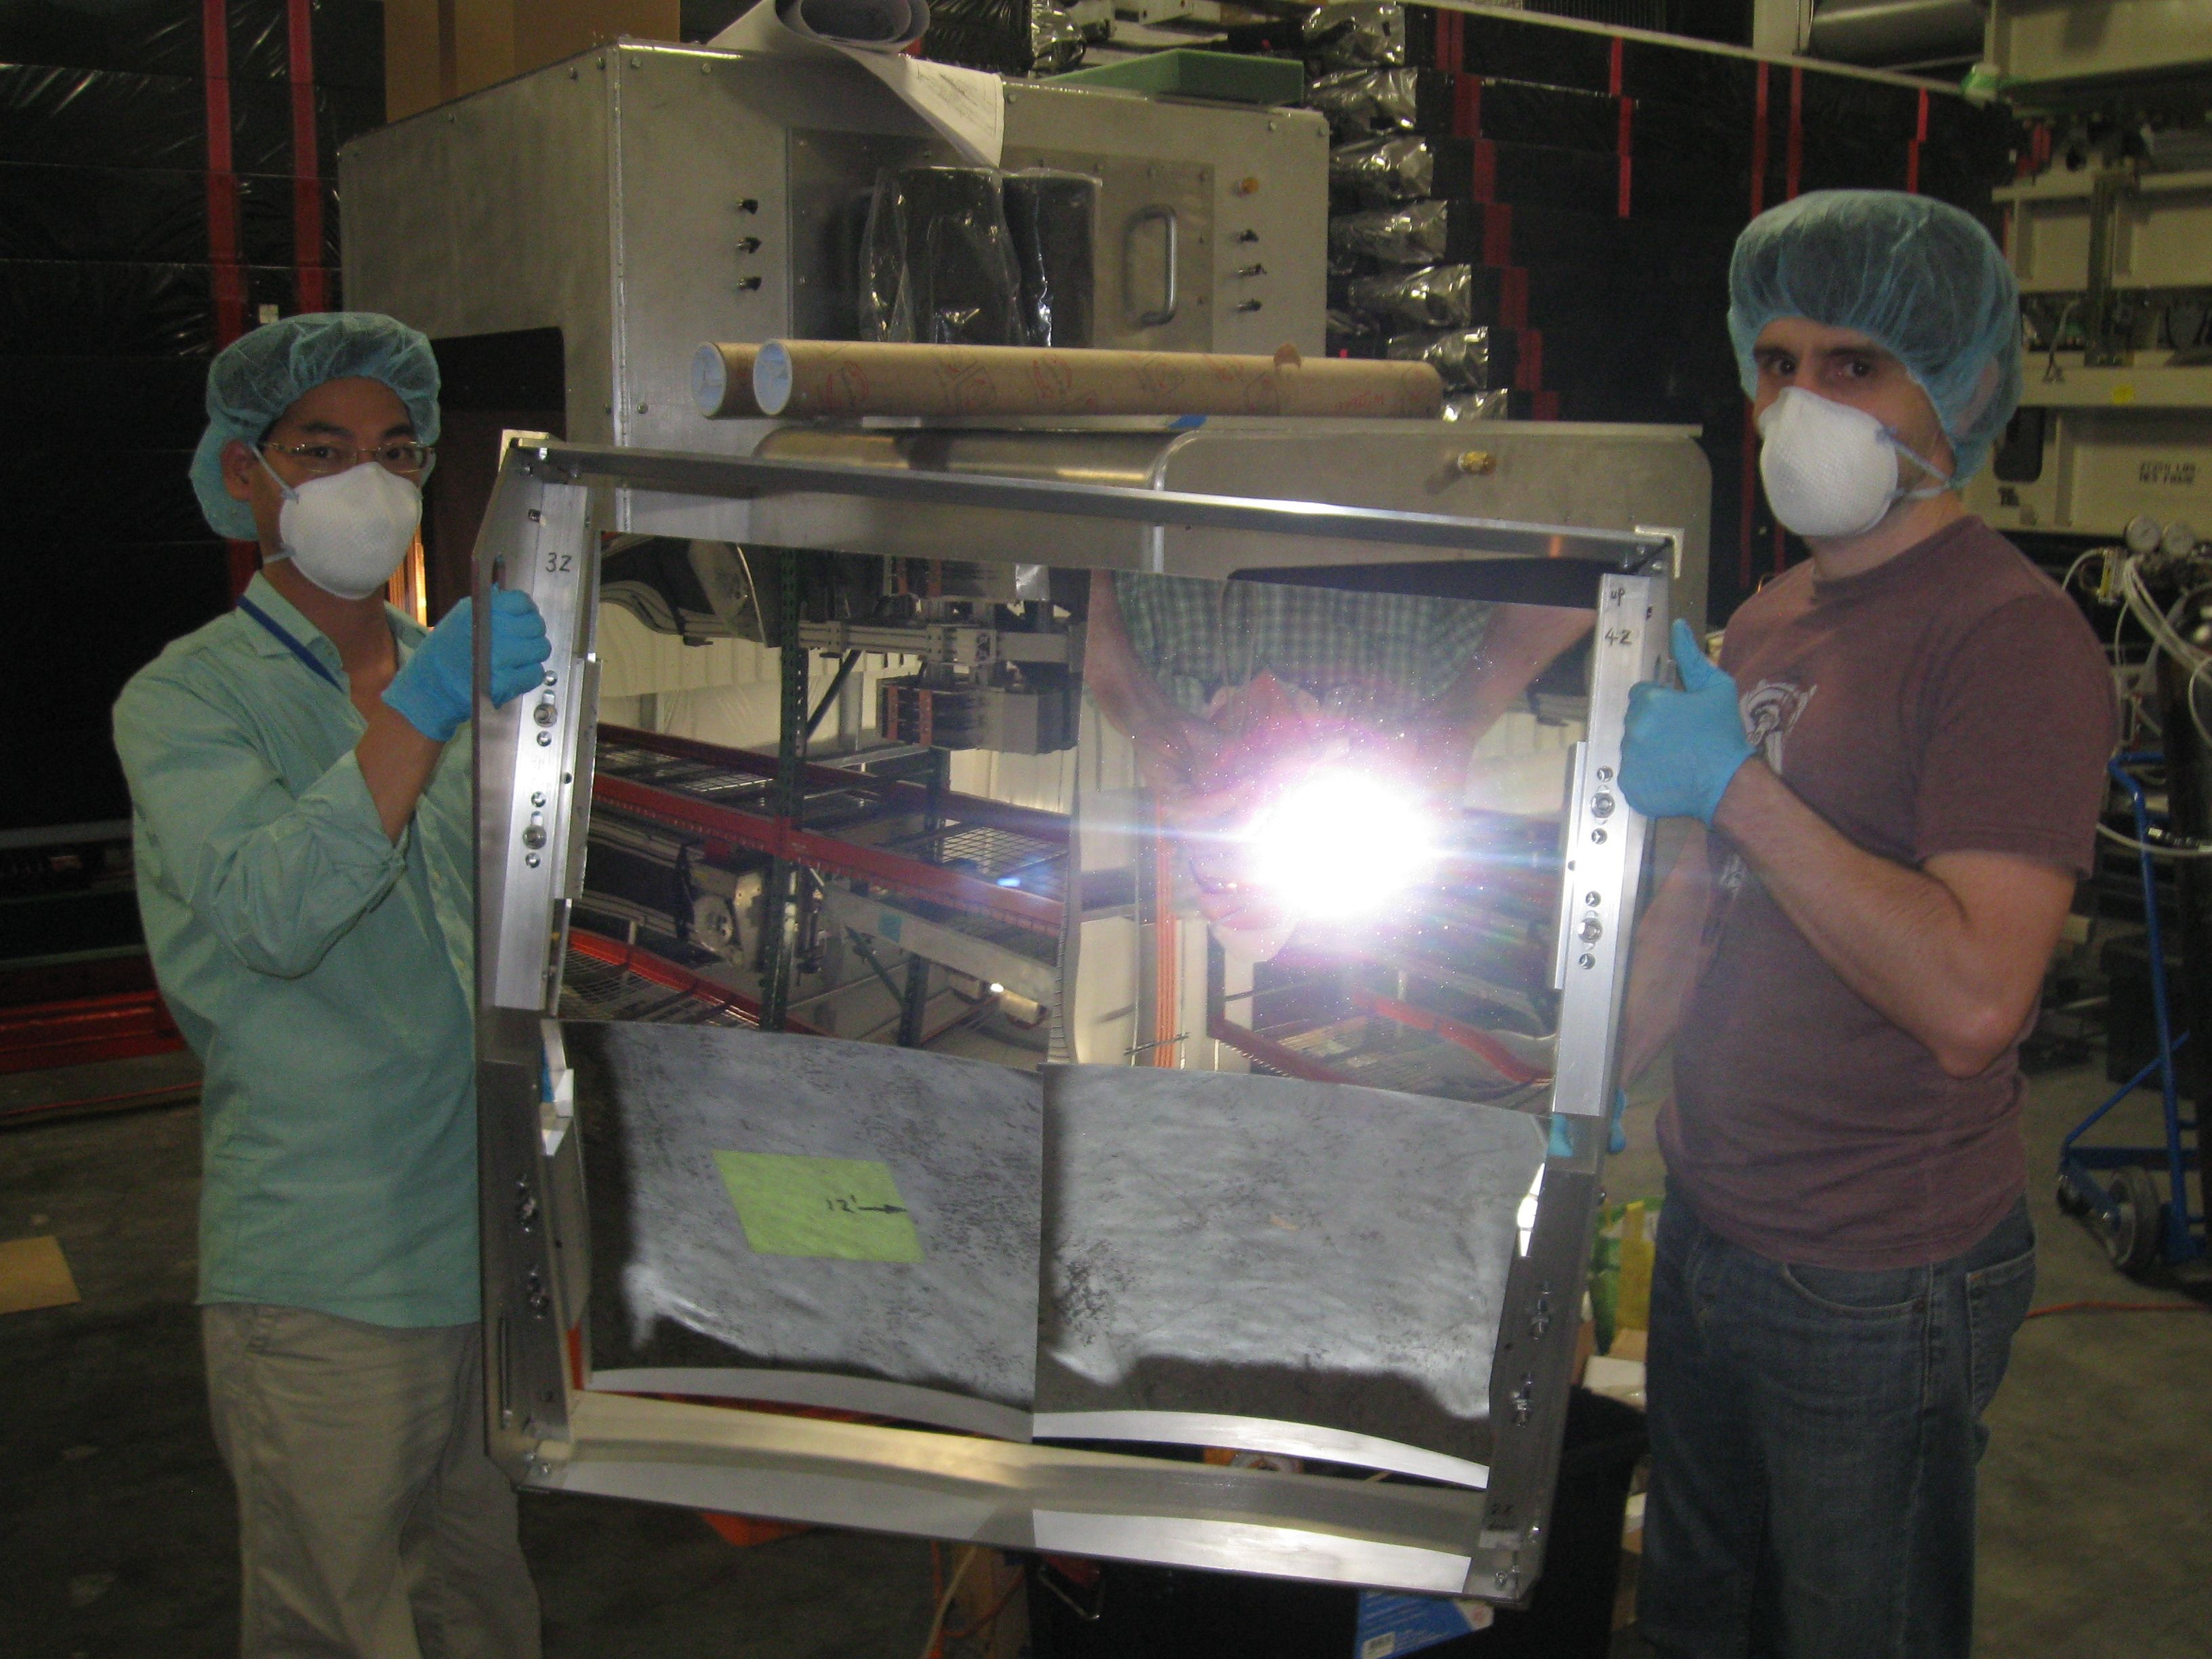
\includegraphics[width=0.45\textwidth]{./Figures/GoingIn} 
   \caption{LHS: Three of four mirrors installed in frame. RHS: Frame about to be moved into tank.\label{fig:install}}
   
   \end{figure}
\end{document}

\paragraph{Operation Procedures}

%\begin{figure}
%%\GHS
%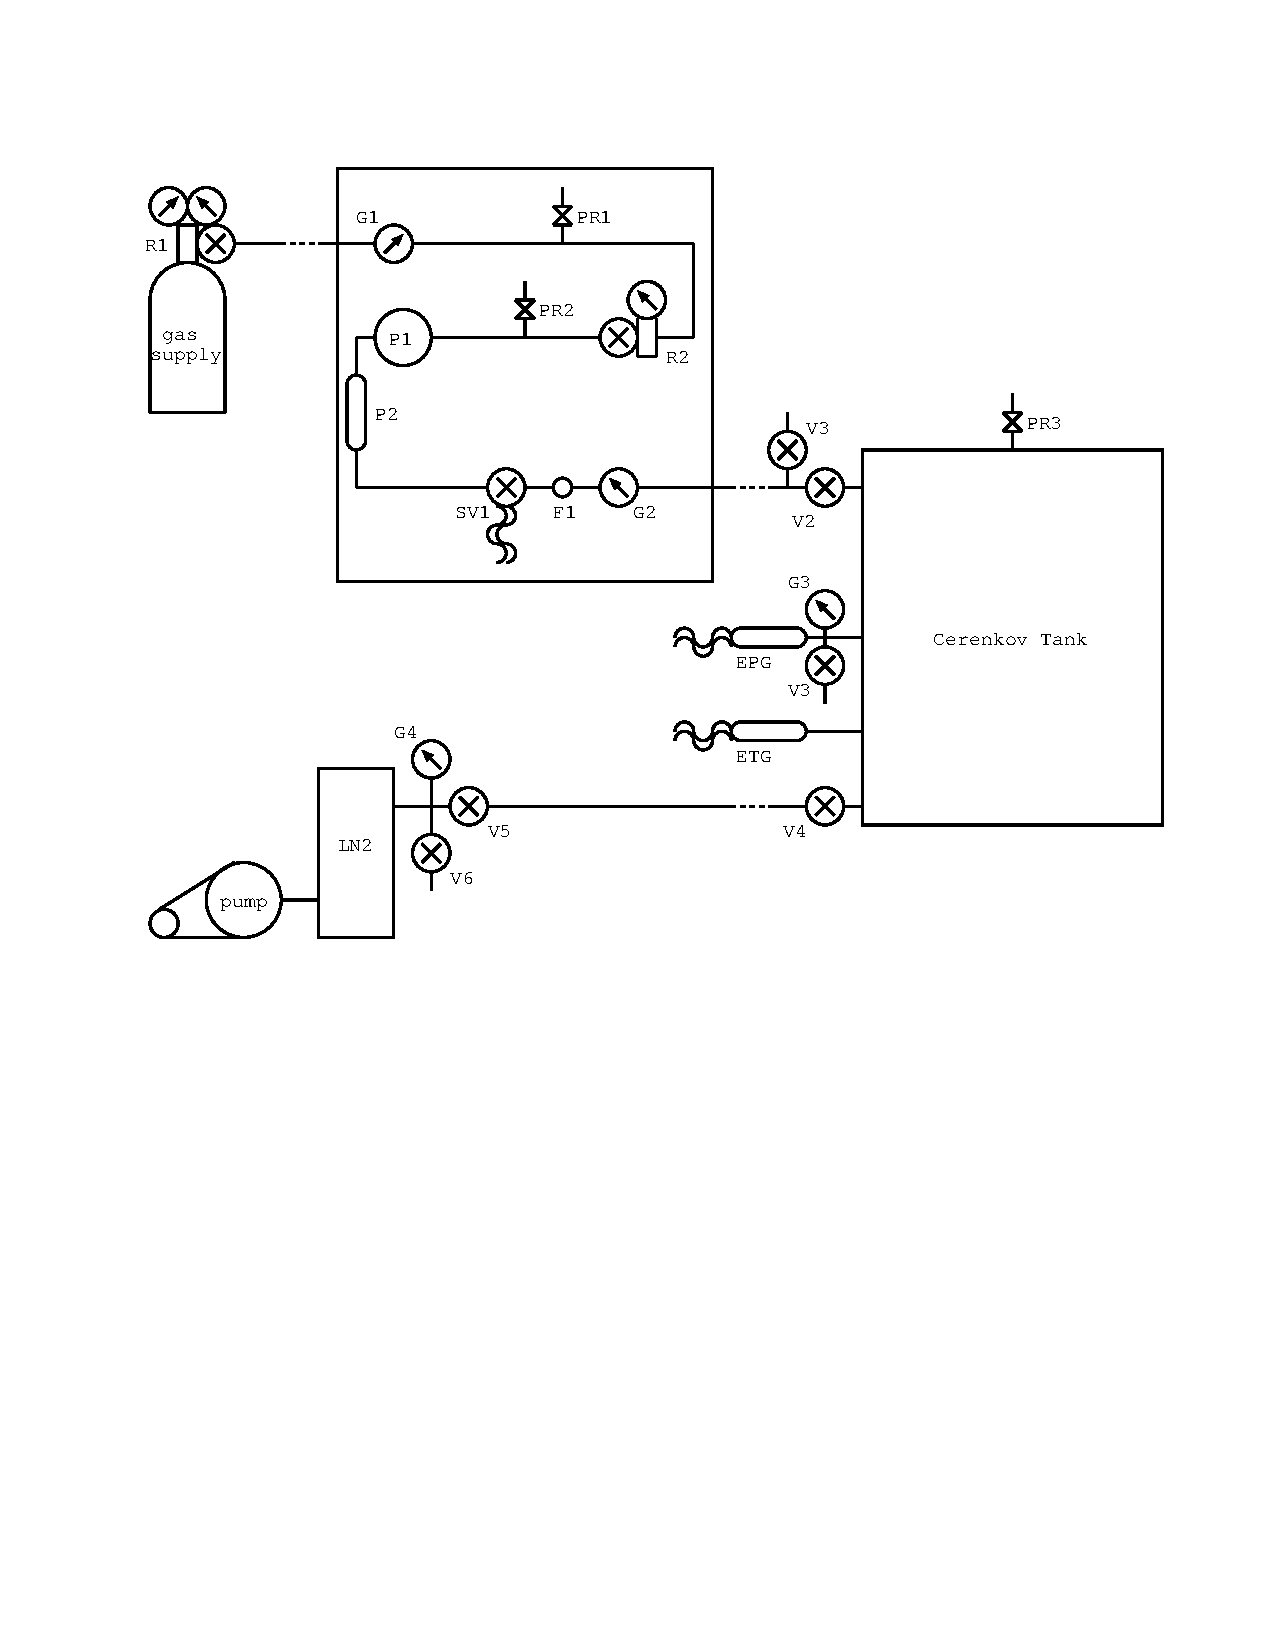
\includegraphics[height=5in,width=6in]{HMSgasC.pdf}
%\caption{The Gas Handling System for the HMS \Cerenkov\ Detector. \label{fig:gas}}
%\end{figure}

The HMS Cerenkov Detector operates either as an e/$\pi$ or $\pi$/p
discriminator. Each mode has a unique set of procedures to prepare the tank
for operation. The nomenclature used in the description of these operation
procedures refers to Figure~\ref{fig:gas}, showing the gas handling system. Components 
shown
inside the dashed box of Figure~\ref{fig:gas}, are all located on the Gas Control Panel.

\paragraph{e/$\bf{\pi}$ Procedures}
For both e/$\bf{\pi}$ and p/$\bf{\pi}$ separation, the procedure 
has been to run with 0.4 to
0.9 (?) atmospheres of C4F10.  This is just a small modifiction to the
current p/pi procedures write-up described in the next section,
with the HMS running sub-atmospheric instead of supra-atmospheric. 

e/$\bf{\pi}$ running can also be accomplished using a nitrogen fill.
This mode of operation requires the tank to be filled with approximately
13.5~psia of $\rm{N_2}$.  The boiloff from the spectrometer magnets is a
perfect source of clean, dry Nitrogen, and is normally used to fill the
Cerenkov tank.

Because the operating pressure is slightly subatmospheric, a pump and fill
procedure is employed.  First make sure that:
\begin{itemize}
\item The 40~mil windows are installed and oriented such that they curve
towards the interior of the tank.
\item Valves {\bf V1-V6} are closed.
\item The LN2 trap is filled.
\item There is enough oil in the pump.
\end{itemize}
The tank is now ready to be evacuated.
\begin{itemize}
\item Turn on the pump.
\item Slowly open {\bf V5}.  This evacuates the pump line.
\item Very slowly open {\bf V4}.  Since this valve connects the pump line to
the detector volume, the pump will work very hard.  Meter this valve
so that the pump is never under extreme stress.  It will take approximately
20~minutes to pump down the tank.
\end{itemize}
The tank can now be filled.
\begin{itemize}
\item Locate the boiloff manifold on the walkway on the top level of the
spectrometer, at the gap between Q3 and the dipole.
\item Turn the valve on this manifold open slightly so that the flow meter
barely registers a flow.
\item Connect the remaining end of the Tygon tubing to the vent of valve
{\bf V3} with a hose clamp.
\item Open valve {\bf V3}.
\item Increase the flow on the flow meter.  Do not exceed 100~cfpm.
\item When {\bf G3} or {\bf EPG} reach the operating pressure, close
the manifold valve.
\item Close {\bf V3}.
\end{itemize}
The fill should take approximately 30 minutes.  The detector should NEVER
be left unattended during a fill.  Frequently check the pressure in the tank
and be aware when the pressure nears one atmosphere.  DO NOT let the pressure
exceed one atmosphere under any circumstances; doing so risks damage to all of
the equipment and personnel in the detector hut.  This pump/fill procedure is usually 
repeated at least once to insure the
purity of the gas.

\paragraph{$\bf{\pi}$/p Procedures}
This mode of operation typically requires the tank to be filled with Freon-12
at pressures varying from 2 to 3~atm.  Because these operating pressures are
greater than 1~atm, the detector must be filled by dilution.  Contamination
from air, however, is not a major problem as the optical absorption properties
of air are actually more favorable than those of Freon-12 itself; the only
difficulty is the increase in pressure needed for a mixture of air and Freon
to achieve the same pion momentum threshold as for a pure sample of Freon.

First prepare the gas handling system:
\begin{itemize}
\item Make sure that the 60~mil windows are installed and oriented such that
they bulge outwards from interior of the tank.
\item Close the valves {\bf V2-V4}, and the valve on regulator {\bf R1}.
{\bf V1}, {\bf SV1}, and the valve on regulator {\bf R2} should be
open.
\item Open the valve on the gas supply bottle.
\item Adjust {\bf R1} to approximately 60 psig.
\item Open the valve on {\bf R1}.
\item Check to make sure gauge {\bf G1} agrees with the pressure setting
on {\bf R1}.
\item Adjust {\bf R2} so that a small flow is detected out the vent of
{\bf V1}.
\item Close {\bf V1}.
\item Adjust {\bf R2} to regulate at the required operating pressure.
\end{itemize}
The tank is now ready for the dilution process.  These steps should be
repeated as few times as possible to minimize the quantity of Freon-12 emitted
to the atmosphere.
\begin{itemize}
\item Record the tank pressure.
\item Open valve {\bf V2}.
\item Monitor the gas pressure until it reaches the required operating pressure.
NEVER let the pressure in the detector exceed 3~atmospheres.
\item Record the final pressure.
\item Open {\bf V3} to vent the tank.
\end{itemize}
From the recorded pressure readings, the threshold momentum of the mixture
of air and Freon-12 can be calculated (assuming the volume of the tank is
fixed).

\end{document}  
